\documentclass[10pt,letterpaper]{article}
\usepackage[margin=.65in]{geometry}
\usepackage[T1]{fontenc}
\usepackage{lmodern,graphicx,booktabs,array}
\usepackage[hidelinks]{hyperref}
\usepackage{fancyhdr}
\pagestyle{fancy}\fancyhf{}\fancyhead[L]{KUKA selective comparisons --- PARTIAL}\fancyhead[R]{16 October 2026}\fancyfoot[C]{\thepage}
\setlength{\headheight}{14pt}\setlength{\parindent}{0pt}\setlength{\parskip}{6pt}\setlength{\emergencystretch}{2em}
\begin{document}
\section*{Selective accounting and matched governor comparisons}
20/32 trials completed; stopped trials remain in the figures. In the primary TCP block, K4 completed 18 s, reduced net human output by 60.9\% relative to K0, and reached 0.148221 W peak human output. Its maximum 10 N force error was 1.647 N and contact absence was 0.00000 s. It achieved 87.3\% of K0 measured progress in the same 18 s. K3 stopped at 10.754 s; this supports a completion benefit for the governor on this fixture, not a measured K3 post-release recovery peak.\par
Both K3 and K4 complete the helping/blocking case. From its 11.7 s release through 18 s, K3/K4 peak x speed is 0.056434/0.064006 m/s and maximum 10 N force error is 0.113279/1.416587 N. K4 reduces post-release reference debt from 18.303 to 13.370 mm and gross human output from 0.123659 to 0.081788 J, but increases those recovery peaks. The reference paper's smoother-recovery claim is therefore not reproduced by this governor adaptation.\par
These are new closed-loop KUKA comparisons inspired by the previous 2-DOF reference. K0 nominal; K1 whole monitored port; K2 residual only; K3 H/R plus human peak power, governor OFF; K4 identical K3 QP, governor ON. The actual plant and nominal 10 N controller are unchanged. A separate contact model evaluates predicted task work at each actual state. Only its explicit tip/table tangential friction changes (1 versus .20). Seven joint torques and a virtual reference clock adapt the reference architecture; they are not its original two-variable Cartesian controller or spatial-anchor governor.\par
\begin{center}\begin{tabular}{llll}\toprule Mode & Protected accounts & Human peak & Governor\\\midrule K0 & monitored only & none & off\\ K1 & whole W & none & off\\ K2 & residual R & none & off\\ K3 & H and R & .15 W & off\\ K4 & same K3 QP & .15 W & on\\\bottomrule\end{tabular}\end{center}
This is deterministic simulation evidence, not a mathematical proof of general safety or reproduction of the reference paper's numerical results. Prediction uses true-plant dynamics with current measured force held for 1 ms; the task model alone is mismatched. The terminal human guard assumes force increments no greater than 60 N/s times 1 ms. Finite-difference rows are checked by fresh nonlinear rollouts; stopped cases expose solver, nonlinear acceptance, or local feasibility limits. No verified fallback, hardware execution, continuous-time certificate, or universal task-preservation claim is made. Gross outgoing energy is not bounded by a net-work account. K3/K4 have no Stage 2 reserve/backup or hard contact-quality constraints.\par
\textbf{Parameters and audit.} H/R/W initial=(.12,.30,.30) J; caps=(.15,.30,.30) J; floors=0; CBF rate=5/s; safe-energy offset=25 microjoules. Four .25 ms physics steps per held 1 ms torque. Central FD=.02 Nm, task weight=1, hard rows and nonlinear acceptance. K4 pauses after an H-triggered intervention and resumes below .02 N measured force, with .1 s clock transitions.
Independent raw-array audit: PASS; regression suite: 91 tests, 0 failures, 0 errors. An audit PASS checks implementation consistency; stopped trials remain failures to complete.\par
\textbf{Provenance.} Source commit \texttt{dfc09dfcb402}. Source SHA256: \texttt{b98d443a9e4b0acf376dd5ba02f0cb2f}\\\texttt{2e0b5a1fca5ac9f5d1bee90c3ecf319b}. Frozen design/configuration, raw data, audit and reproduction commands accompany this PDF.
\clearpage\section*{All primary comparisons}
\begingroup\small\setlength{\tabcolsep}{3pt}\begin{center}\begin{tabular}{llrrrrrrr}\toprule Case & Mode/end s & H net J & min H J & min R J & Peak W & Force err N & Loss s & QPs\\\midrule
A & K0/18.000 & -0.00000 & 0.12 & 0.3 & 0.0000 & 0.05 & 0.0000 & 0 \\
A & K1 STOP/12.541 & -0.00000 & 0.12 & 0.3 & 0.0000 & 1.85 & 0.0000 & 3229 \\
A & K2/18.000 & -0.00000 & 0.12 & 0.3 & 0.0000 & 0.05 & 0.0000 & 0 \\
A & K3/18.000 & -0.00000 & 0.12 & 0.3 & 0.0000 & 0.05 & 0.0000 & 0 \\
A & K4/18.000 & -0.00000 & 0.12 & 0.3 & 0.0000 & 0.05 & 0.0000 & 0 \\
B & K0/18.000 & -0.00000 & 0.12 & 0.06704 & 0.0000 & 0.05 & 0.0000 & 0 \\
B & K1 STOP/12.541 & -0.00000 & 0.12 & 0.2149 & 0.0000 & 1.85 & 0.0000 & 3229 \\
B & K2/18.000 & -0.00000 & 0.12 & 0.06704 & 0.0000 & 0.05 & 0.0000 & 0 \\
B & K3/18.000 & -0.00000 & 0.12 & 0.06704 & 0.0000 & 0.05 & 0.0000 & 0 \\
B & K4/18.000 & -0.00000 & 0.12 & 0.06704 & 0.0000 & 0.05 & 0.0000 & 0 \\
C & K0/18.000 & 0.18743 & -0.06743 & 0.1126 & 0.2951 & 0.14 & 0.0000 & 0 \\
C & K1 STOP/10.624 & 0.13225 & -0.01225 & 0.1678 & 0.2651 & 3.07 & 0.0000 & 214 \\
C & K2/18.000 & 0.18743 & -0.06743 & 0.1126 & 0.2951 & 0.14 & 0.0000 & 0 \\
C & K3 STOP/10.754 & 0.10917 & 0.01083 & 0.1908 & 0.1482 & 14.75 & 0.0000 & 588 \\
C & K4/18.000 & 0.07321 & 0.04679 & 0.2268 & 0.1482 & 1.65 & 0.0000 & 40 \\
\bottomrule\end{tabular}\end{center}\endgroup\par
A: exact/no human; B: mismatch/no human; C: TCP block; D: mismatch plus TCP block; E: forearm block; F: help then block; S: starved H. Force error is measured relative to the original 10 N target over the available 8.71 s onward window. Totals from stopped prefixes must not be read as complete-run savings. Negative unprotected account values remain visible.\par
A\_exact\_nohuman/K1: stopped at 12.541 s: nonlinear\_retries\_exhausted.\\
B\_mismatch\_nohuman/K1: stopped at 12.541 s: nonlinear\_retries\_exhausted.\\
C\_blocking/K1: stopped at 10.624 s: solver\_failure.\\
C\_blocking/K3: stopped at 10.754 s: nonlinear\_retries\_exhausted.\\
\clearpage\section*{Remaining comparisons and challenge}
\begingroup\small\setlength{\tabcolsep}{3pt}\begin{center}\begin{tabular}{llrrrrrrr}\toprule Case & Mode/end s & H net J & min H J & min R J & Peak W & Force err N & Loss s & QPs\\\midrule
D & K0/18.000 & 0.18743 & -0.06743 & -0.2145 & 0.2951 & 0.14 & 0.0000 & 0 \\
D & K1 STOP/10.624 & 0.13225 & -0.01225 & 0.1379 & 0.2651 & 3.07 & 0.0000 & 214 \\
D & K2 STOP/10.752 & 0.17110 & -0.0511 & 0.07536 & 0.2951 & 0.20 & 0.0000 & 48 \\
D & K3 STOP/10.754 & 0.10917 & 0.01083 & 0.1839 & 0.1482 & 14.75 & 0.0000 & 588 \\
D & K4 STOP/14.948 & 0.07321 & 0.04679 & 0.01367 & 0.1482 & 1.65 & 0.0000 & 153 \\
E & K0/18.000 & 0.24162 & -0.1216 & 0.05838 & 0.2389 & 0.40 & 0.0000 & 0 \\
E & K1 STOP/10.335 & 0.13227 & -0.01227 & 0.1677 & 0.2442 & 3.02 & 0.0000 & 242 \\
E & K2/18.000 & 0.24162 & -0.1216 & 0.05838 & 0.2389 & 0.40 & 0.0000 & 0 \\
E & K3 STOP/10.232 & 0.08897 & 0.03103 & 0.211 & 0.1482 & 5.08 & 0.0000 & 655 \\
E & K4/18.000 & 0.03914 & 0.07605 & 0.2561 & 0.1482 & 0.93 & 0.0000 & 10 \\
F & K0/18.000 & 0.02531 & 0.01173 & 0.1617 & 0.1899 & 0.25 & 0.0000 & 0 \\
F & K1 STOP/13.715 & 0.02213 & 0.0149 & 0.1649 & 0.1899 & 3.87 & 0.0000 & 3721 \\
F & K2/18.000 & 0.02531 & 0.01173 & 0.1617 & 0.1899 & 0.25 & 0.0000 & 0 \\
F & K3/18.000 & 0.01069 & 0.02634 & 0.1763 & 0.1482 & 0.29 & 0.0000 & 383 \\
F & K4/18.000 & -0.03118 & 0.06821 & 0.2182 & 0.1482 & 1.42 & 0.0000 & 31 \\
S & K3 STOP/10.363 & 0.00094 & 5.566e-05 & 0.2991 & 0.0041 & 17.48 & 0.0000 & 1263 \\
S & K4/18.000 & -0.06573 & 0.000683 & 0.2938 & 0.0291 & 11.05 & 0.0000 & 60 \\
\bottomrule\end{tabular}\end{center}\endgroup\par
A: exact/no human; B: mismatch/no human; C: TCP block; D: mismatch plus TCP block; E: forearm block; F: help then block; S: starved H. Force error is measured relative to the original 10 N target over the available 8.71 s onward window. Totals from stopped prefixes must not be read as complete-run savings. Negative unprotected account values remain visible.\par
D\_combined/K1: stopped at 10.624 s: solver\_failure.\\
D\_combined/K2: stopped at 10.752 s: nonlinear\_retries\_exhausted.\\
D\_combined/K3: stopped at 10.754 s: nonlinear\_retries\_exhausted.\\
D\_combined/K4: stopped at 14.948 s: nonlinear\_retries\_exhausted.\\
E\_forearm\_block/K1: stopped at 10.335 s: solver\_failure.\\
E\_forearm\_block/K3: stopped at 10.232 s: nonlinear\_retries\_exhausted.\\
F\_help\_block/K1: stopped at 13.715 s: nonlinear\_retries\_exhausted.\\
S\_starved/K3: stopped at 10.363 s: nonlinear\_retries\_exhausted.\\
\clearpage\section*{F3 adaptation: predictable task work and whole-port depletion}
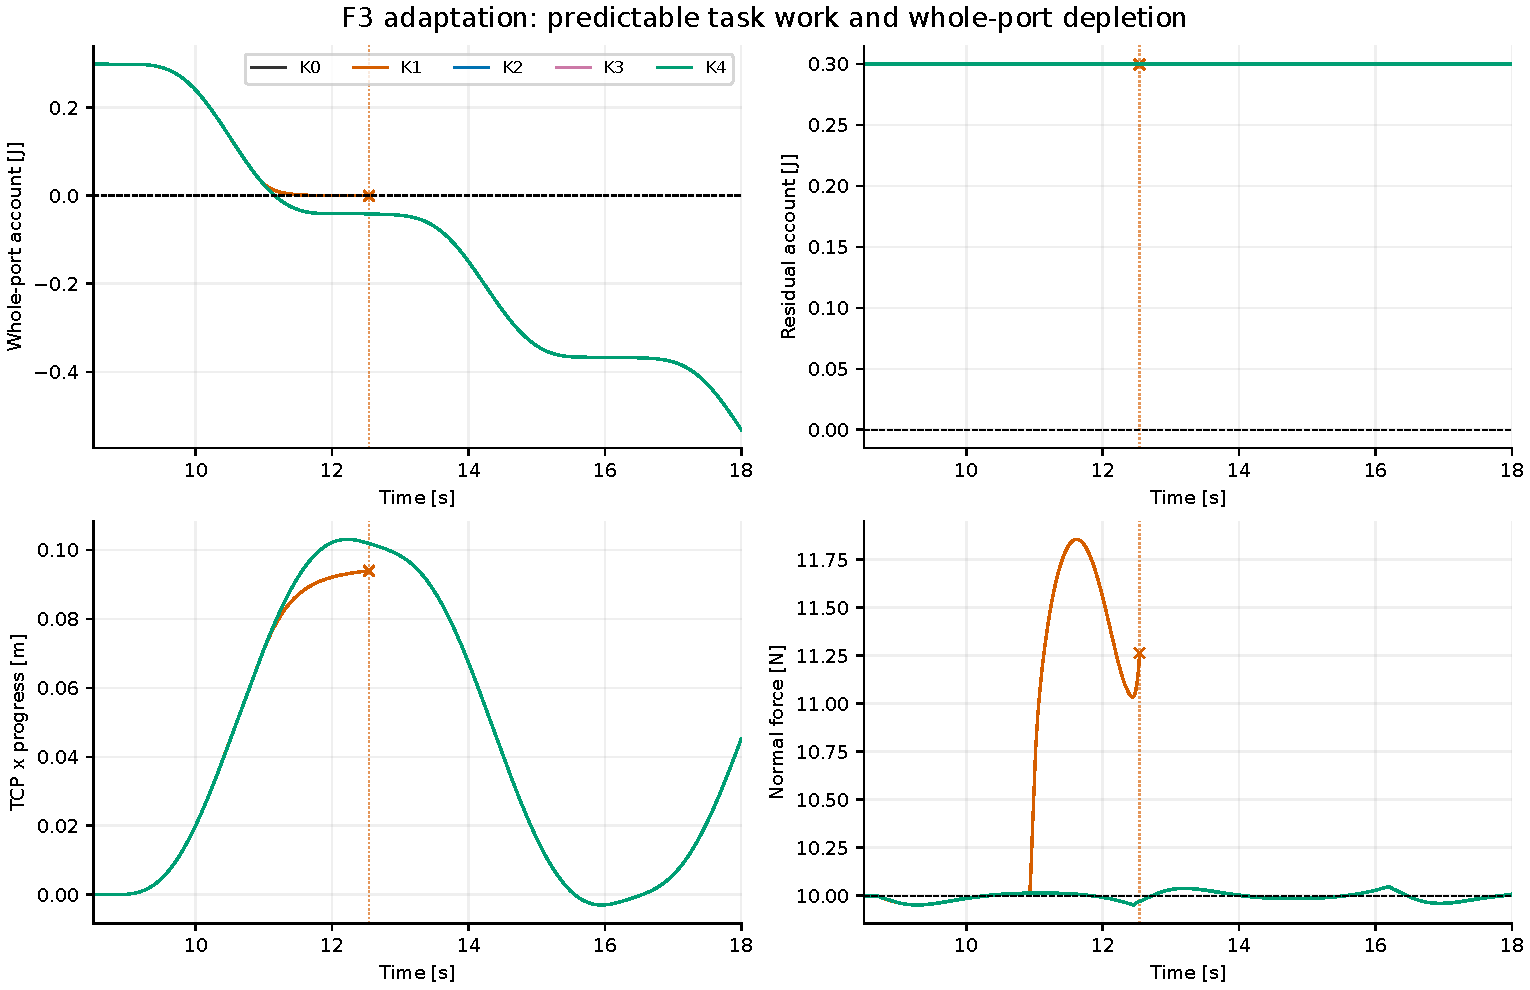
\includegraphics[width=\textwidth]{figures/fig3_exact.pdf}
Exact model, no human. K2/K3/K4 should be transparent; K1 accounts for ordinary task work. Crosses and dotted lines mark explicit stops, never zero-padded continuations.\par
K0: COMPLETE, end 18.000 s; net/gross H output -0.000000/0.000000 J; min H/R 0.12/0.3 J; peak H 0.000000 W; measured progress 0.2453 m; QP attempts 0.\par
K1: STOP, end 12.541 s; net/gross H output -0.000000/0.000000 J; min H/R 0.12/0.3 J; peak H 0.000000 W; measured progress 0.0939 m; QP attempts 3229.\par
K2: COMPLETE, end 18.000 s; net/gross H output -0.000000/0.000000 J; min H/R 0.12/0.3 J; peak H 0.000000 W; measured progress 0.2453 m; QP attempts 0.\par
K3: COMPLETE, end 18.000 s; net/gross H output -0.000000/0.000000 J; min H/R 0.12/0.3 J; peak H 0.000000 W; measured progress 0.2453 m; QP attempts 0.\par
K4: COMPLETE, end 18.000 s; net/gross H output -0.000000/0.000000 J; min H/R 0.12/0.3 J; peak H 0.000000 W; measured progress 0.2453 m; QP attempts 0.\par
\clearpage\section*{F4 adaptation: task-model mismatch without human input}
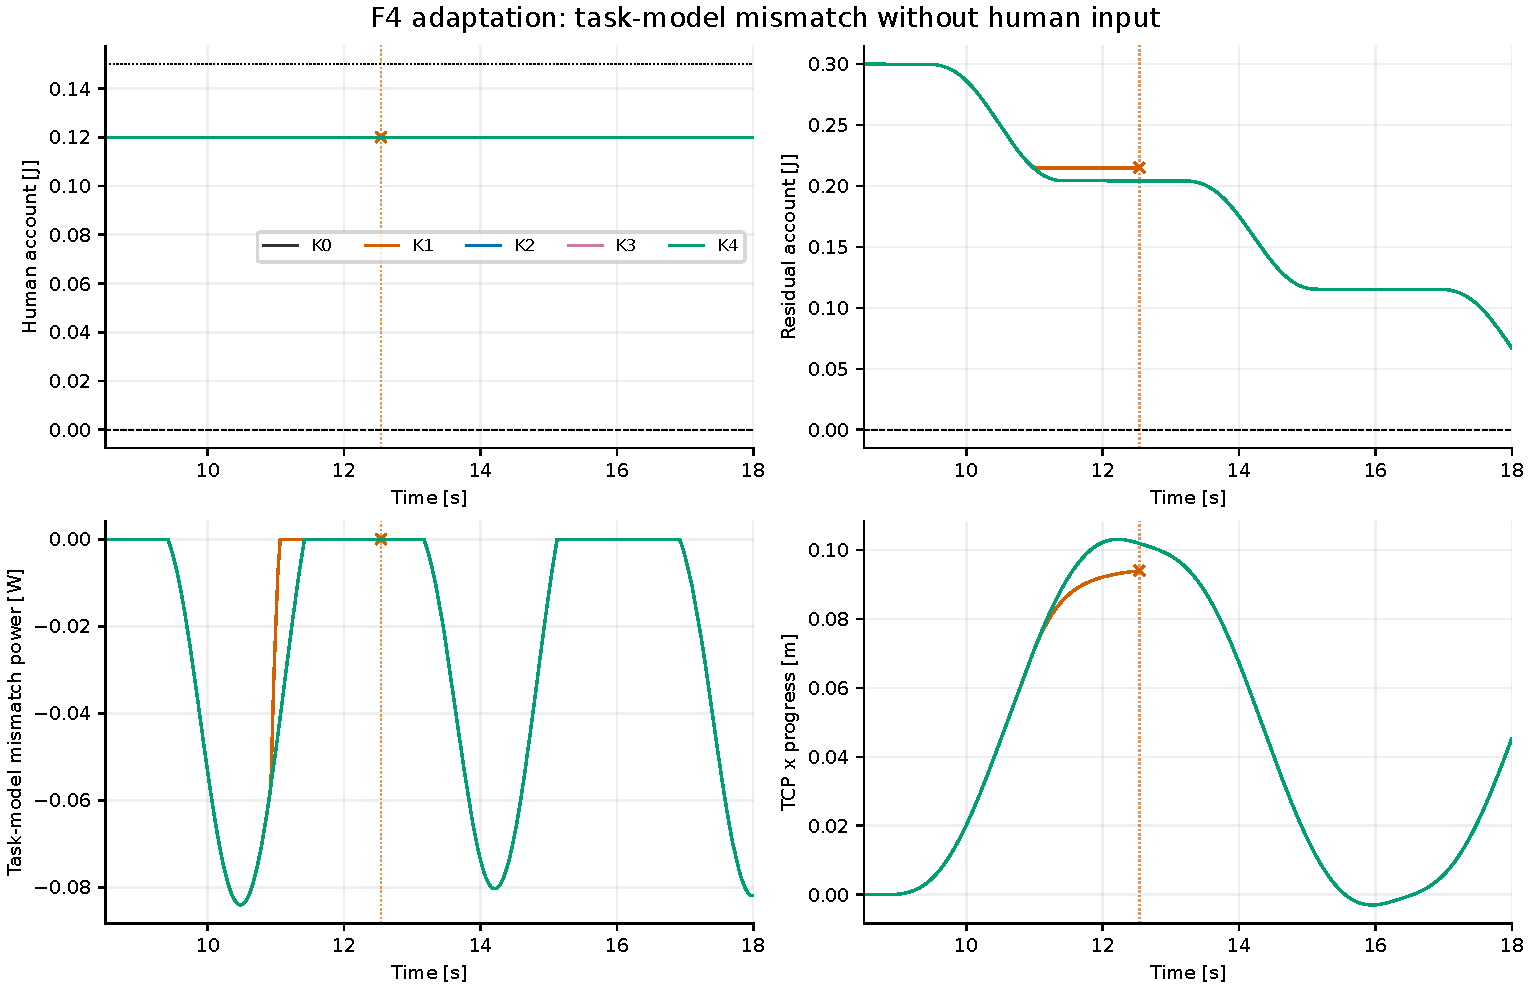
\includegraphics[width=\textwidth]{figures/fig4_mismatch.pdf}
Actual friction remains 1; nominal pair friction is .20. Nonzero residual power with zero human power establishes independent accounting. It does not establish robustness to unknown plant dynamics.\par
K0: COMPLETE, end 18.000 s; net/gross H output -0.000000/0.000000 J; min H/R 0.12/0.0670424 J; peak H 0.000000 W; measured progress 0.2453 m; QP attempts 0.\par
K1: STOP, end 12.541 s; net/gross H output -0.000000/0.000000 J; min H/R 0.12/0.214862 J; peak H 0.000000 W; measured progress 0.0939 m; QP attempts 3229.\par
K2: COMPLETE, end 18.000 s; net/gross H output -0.000000/0.000000 J; min H/R 0.12/0.0670424 J; peak H 0.000000 W; measured progress 0.2453 m; QP attempts 0.\par
K3: COMPLETE, end 18.000 s; net/gross H output -0.000000/0.000000 J; min H/R 0.12/0.0670424 J; peak H 0.000000 W; measured progress 0.2453 m; QP attempts 0.\par
K4: COMPLETE, end 18.000 s; net/gross H output -0.000000/0.000000 J; min H/R 0.12/0.0670424 J; peak H 0.000000 W; measured progress 0.2453 m; QP attempts 0.\par
\clearpage\section*{F5 adaptation: dedicated human energy and peak-power protection}
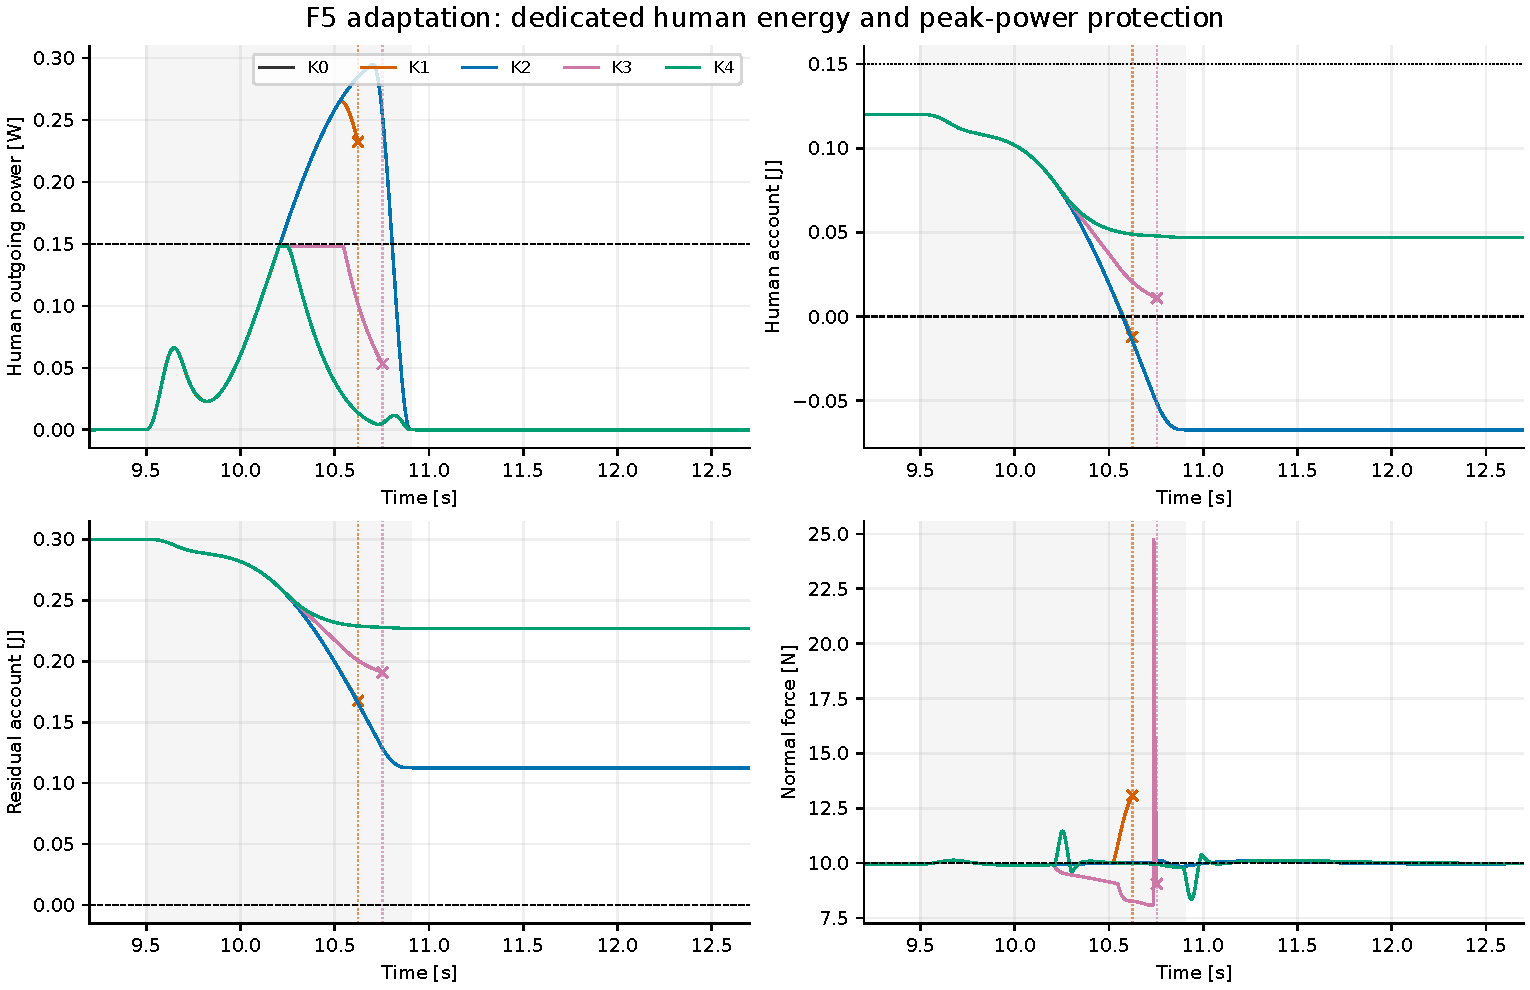
\includegraphics[width=\textwidth]{figures/fig5_human.pdf}
All modes use the same 5 N TCP block. K3/K4 enforce the .15 W human peak bound and H/R rows. K2 has the larger residual budget and no separate H constraint. Compare completion as well as safe prefixes.\par
K0: COMPLETE, end 18.000 s; net/gross H output 0.187435/0.187435 J; min H/R -0.067435/0.112565 J; peak H 0.295100 W; measured progress 0.2455 m; QP attempts 0.\par
K1: STOP, end 10.624 s; net/gross H output 0.132250/0.132250 J; min H/R -0.01225/0.16775 J; peak H 0.265072 W; measured progress 0.0331 m; QP attempts 214.\par
K2: COMPLETE, end 18.000 s; net/gross H output 0.187435/0.187435 J; min H/R -0.067435/0.112565 J; peak H 0.295100 W; measured progress 0.2455 m; QP attempts 0.\par
K3: STOP, end 10.754 s; net/gross H output 0.109175/0.109175 J; min H/R 0.0108255/0.190825 J; peak H 0.148221 W; measured progress 0.0286 m; QP attempts 588.\par
K4: COMPLETE, end 18.000 s; net/gross H output 0.073209/0.073209 J; min H/R 0.0467912/0.226791 J; peak H 0.148221 W; measured progress 0.2143 m; QP attempts 40.\par
\clearpage\section*{F6 adaptation: simultaneous human input and task-model mismatch}
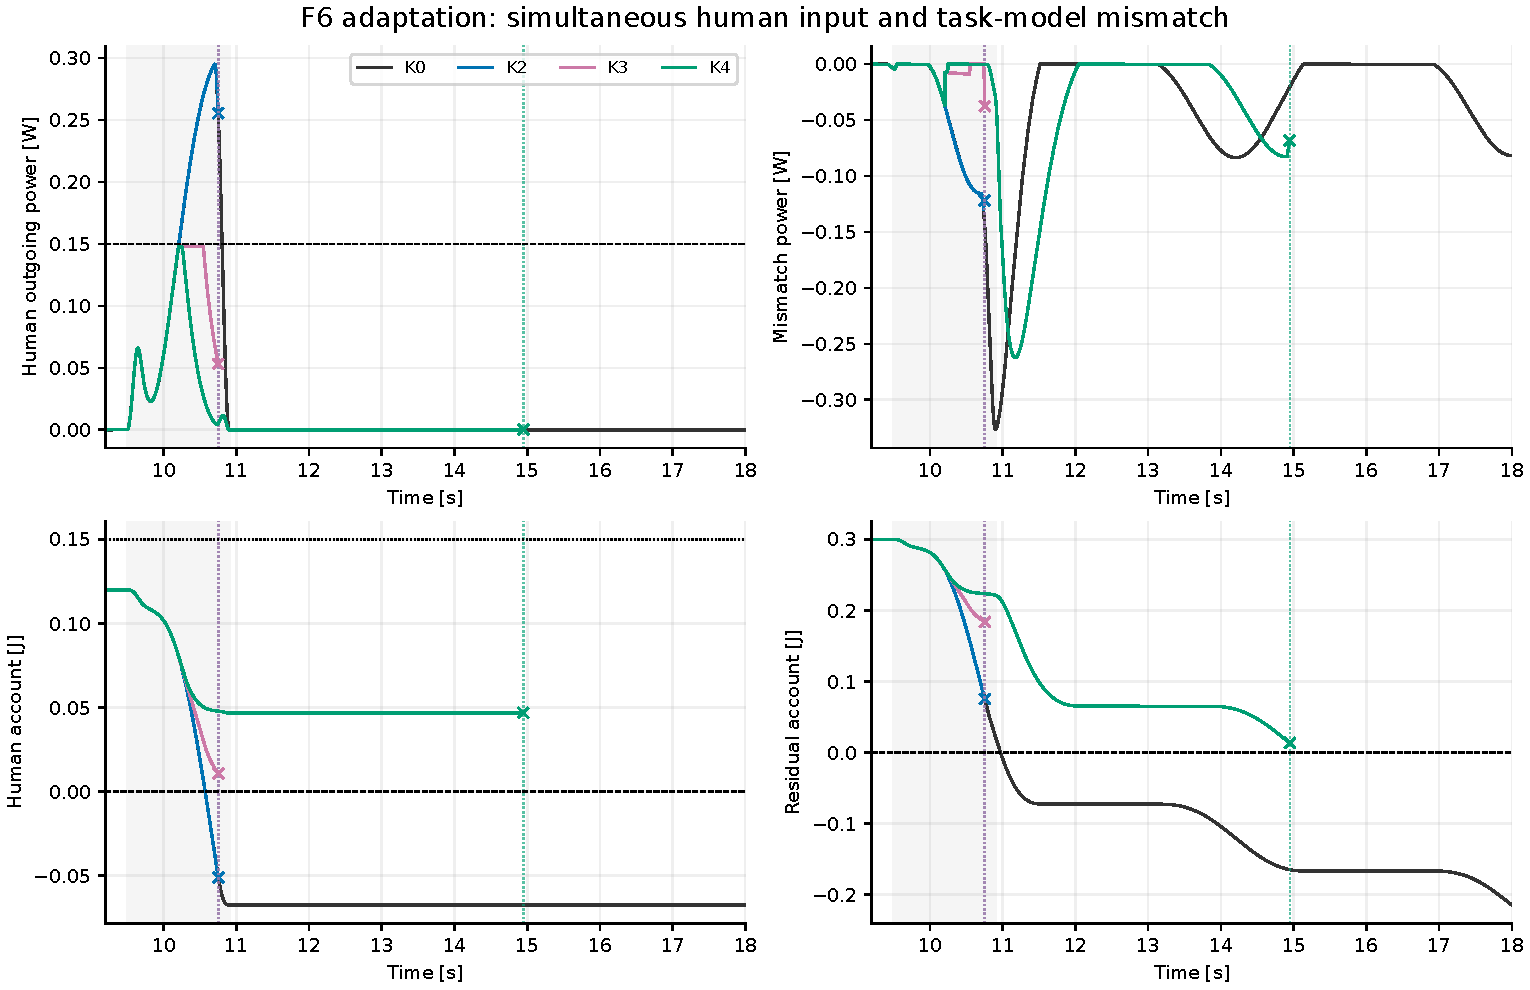
\includegraphics[width=\textwidth]{figures/fig6_combined.pdf}
At every executed sample, pR=pH+(pT-pT\_hat). H and R have independently initialized budgets. The cap is applied separately to each account; the raw reconstruction checks both identities.\par
K0: COMPLETE, end 18.000 s; net/gross H output 0.187435/0.187435 J; min H/R -0.067435/-0.214466 J; peak H 0.295100 W; measured progress 0.2455 m; QP attempts 0.\par
K2: STOP, end 10.752 s; net/gross H output 0.171101/0.171101 J; min H/R -0.0511006/0.0753639 J; peak H 0.295100 W; measured progress 0.0411 m; QP attempts 48.\par
K3: STOP, end 10.754 s; net/gross H output 0.109175/0.109175 J; min H/R 0.0108255/0.183927 J; peak H 0.148221 W; measured progress 0.0286 m; QP attempts 588.\par
K4: STOP, end 14.948 s; net/gross H output 0.073209/0.073209 J; min H/R 0.0467912/0.0136669 J; peak H 0.148221 W; measured progress 0.1452 m; QP attempts 153.\par
\clearpage\section*{F7 adaptation: helping, upper-cap saturation, then blocking}
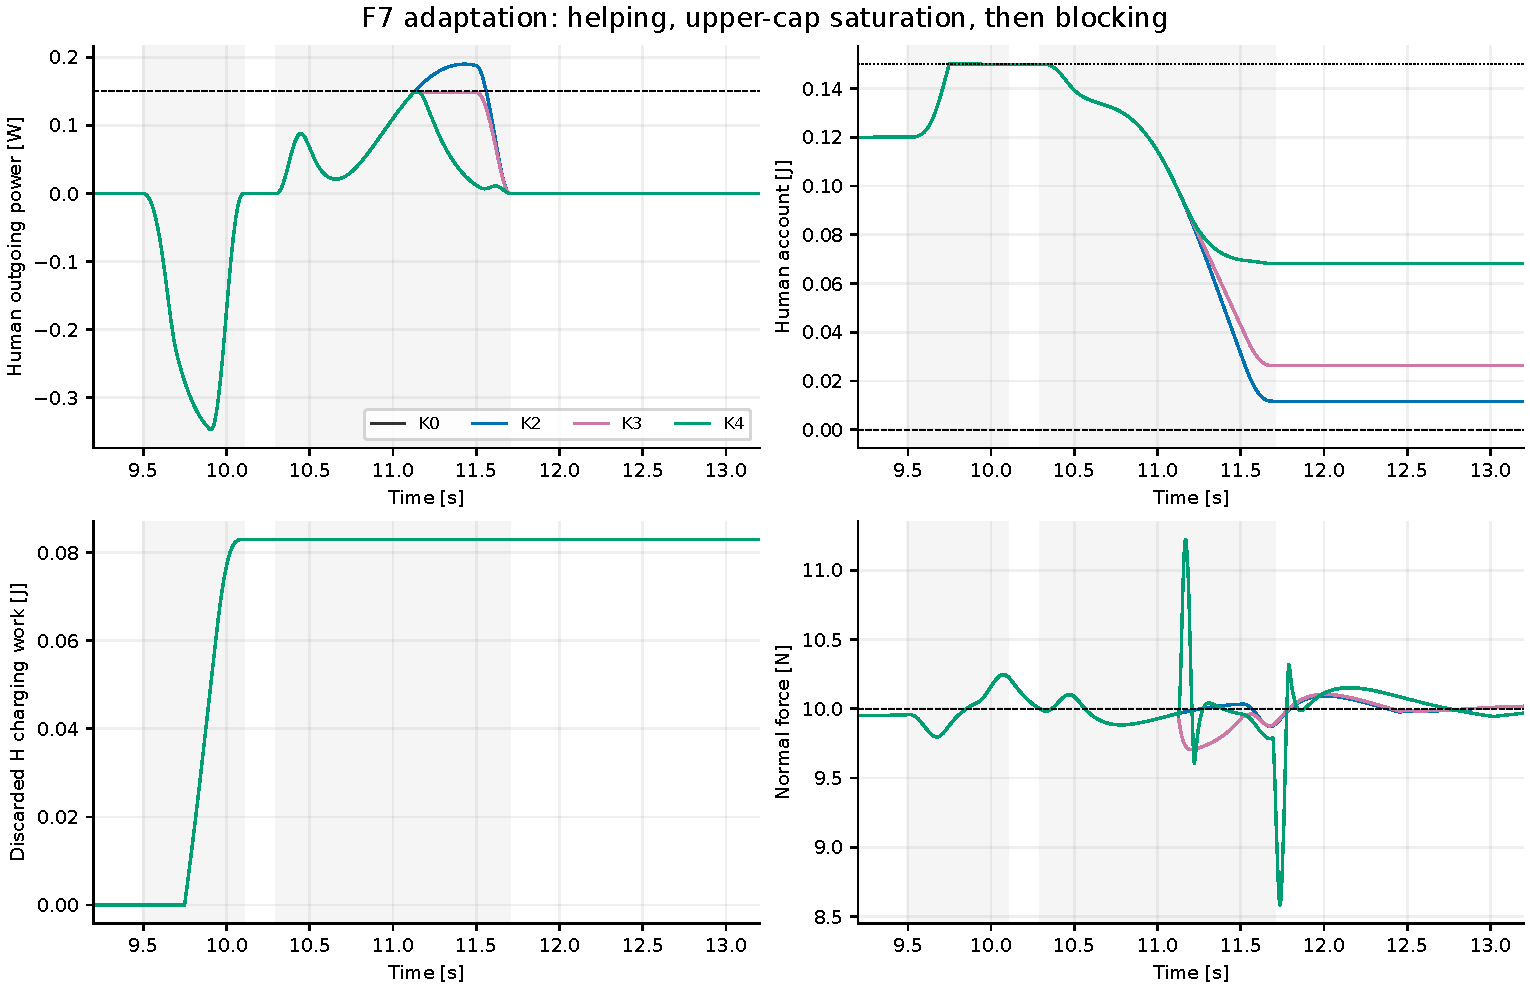
\includegraphics[width=\textwidth]{figures/fig7_charge.pdf}
One continuous trial: helping starts at 9.5 s, blocking at 10.3 s. H charges only to .15 J; discarded charging is explicitly logged. Net outgoing work and gross outgoing work are distinct.\par
K0: COMPLETE, end 18.000 s; net/gross H output 0.025306/0.138273 J; min H/R 0.0117267/0.161727 J; peak H 0.189865 W; measured progress 0.2456 m; QP attempts 0.\par
K2: COMPLETE, end 18.000 s; net/gross H output 0.025306/0.138273 J; min H/R 0.0117267/0.161727 J; peak H 0.189865 W; measured progress 0.2456 m; QP attempts 0.\par
K3: COMPLETE, end 18.000 s; net/gross H output 0.010692/0.123659 J; min H/R 0.0263407/0.176341 J; peak H 0.148221 W; measured progress 0.2455 m; QP attempts 383.\par
K4: COMPLETE, end 18.000 s; net/gross H output -0.031180/0.081788 J; min H/R 0.068212/0.218212 J; peak H 0.148221 W; measured progress 0.2187 m; QP attempts 31.\par
\clearpage\section*{F8 adaptation: matched K3/K4, governor OFF/ON}
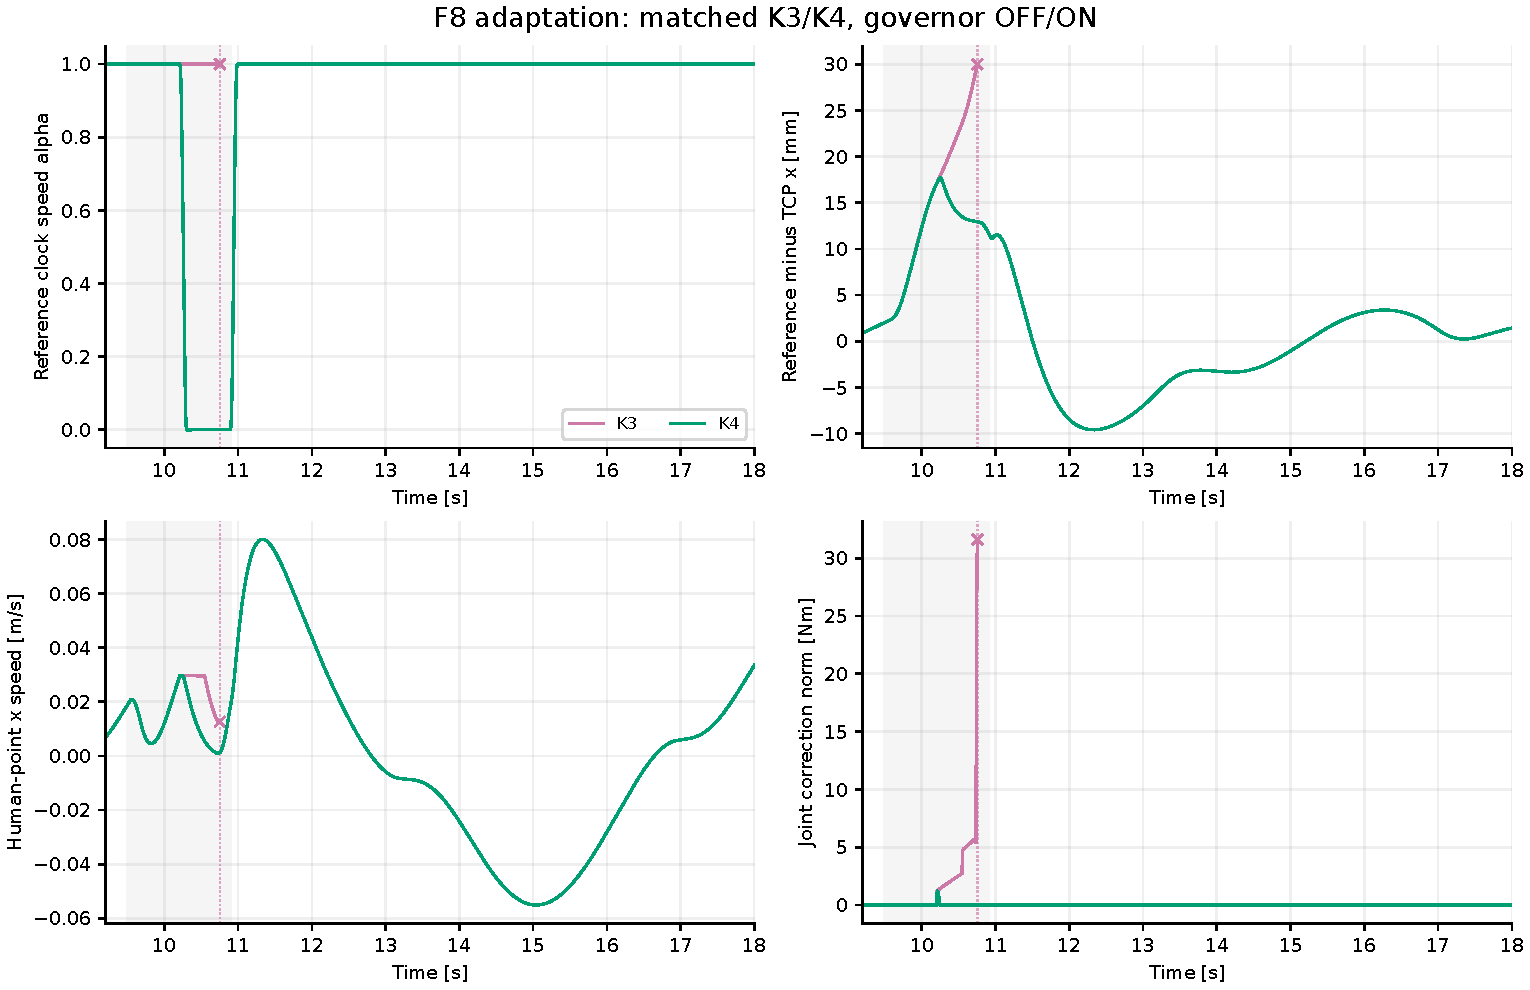
\includegraphics[width=\textwidth]{figures/fig8_governor.pdf}
K3/K4 share the QP, bounds, budgets and model; only the reference-clock governor changes. A stopped K3 trace cannot establish a post-release catch-up peak. Joint correction is not a reconstructed Cartesian command.\par
K3: STOP, end 10.754 s; net/gross H output 0.109175/0.109175 J; min H/R 0.0108255/0.190825 J; peak H 0.148221 W; measured progress 0.0286 m; QP attempts 588.\par
K4: COMPLETE, end 18.000 s; net/gross H output 0.073209/0.073209 J; min H/R 0.0467912/0.226791 J; peak H 0.148221 W; measured progress 0.2143 m; QP attempts 40.\par
\clearpage\section*{Matched governor comparison through helping and blocking}
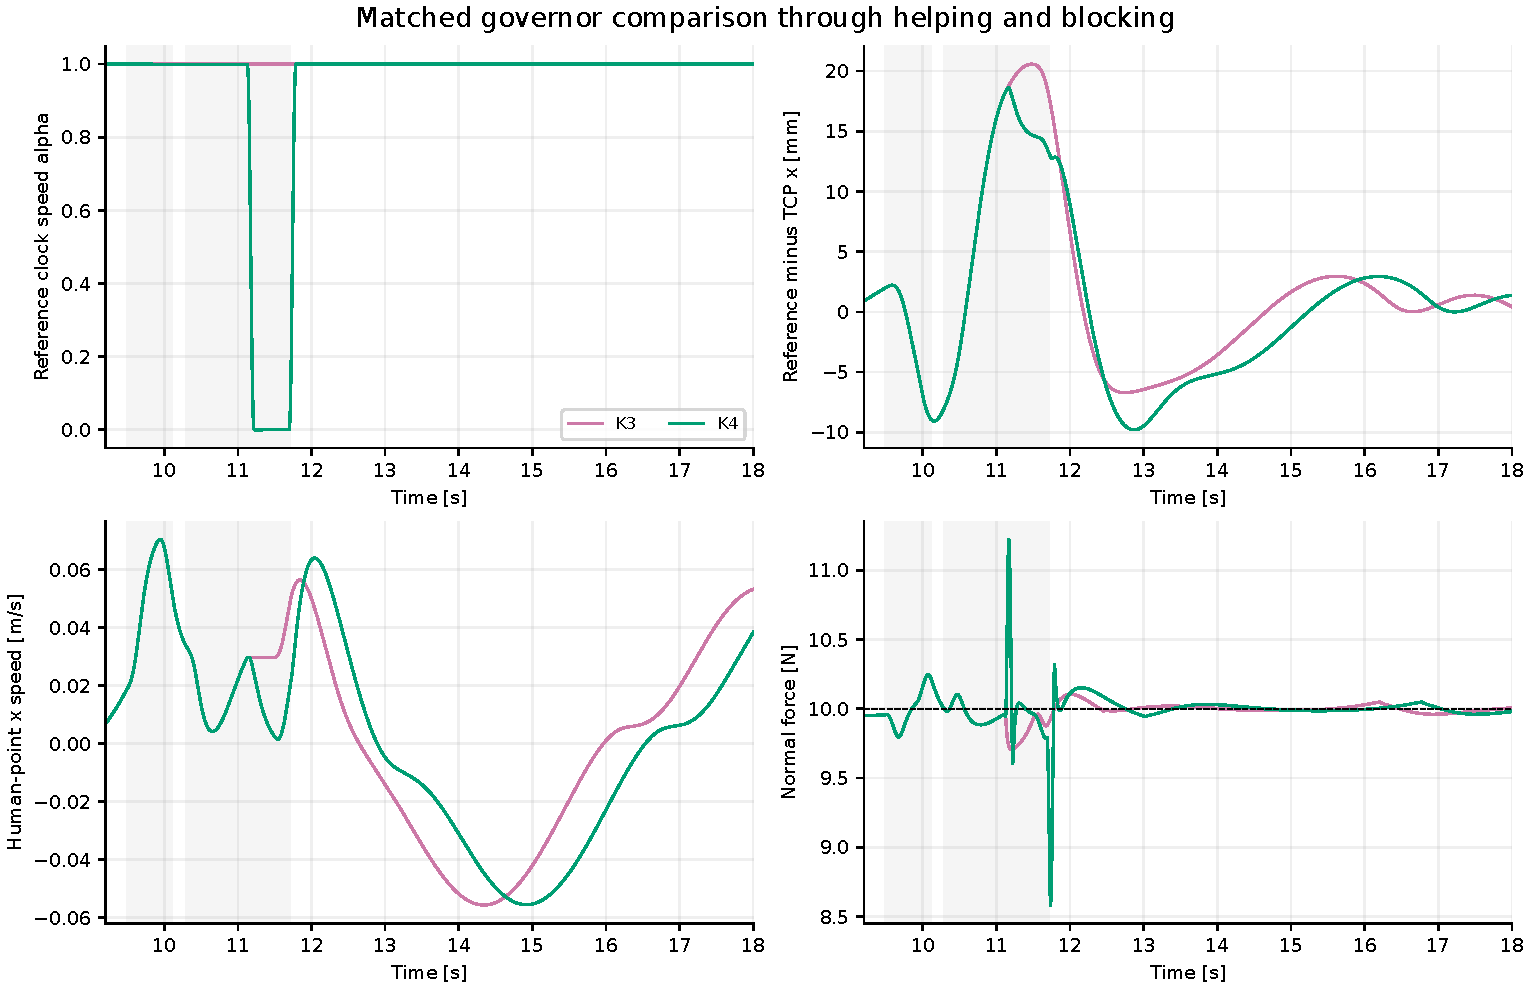
\includegraphics[width=\textwidth]{figures/fig9_help_recovery.pdf}
Both trials complete. After the 11.7 s release, K3/K4 peak x speeds are .056434/.064006 m/s and force errors .113279/1.416587 N. The governor reduces human output and reference debt but worsens these recovery peaks.\par
K3: COMPLETE, end 18.000 s; net/gross H output 0.010692/0.123659 J; min H/R 0.0263407/0.176341 J; peak H 0.148221 W; measured progress 0.2455 m; QP attempts 383.\par
K4: COMPLETE, end 18.000 s; net/gross H output -0.031180/0.081788 J; min H/R 0.068212/0.218212 J; peak H 0.148221 W; measured progress 0.2187 m; QP attempts 31.\par
\clearpage\section*{Second human port: forearm rather than TCP}
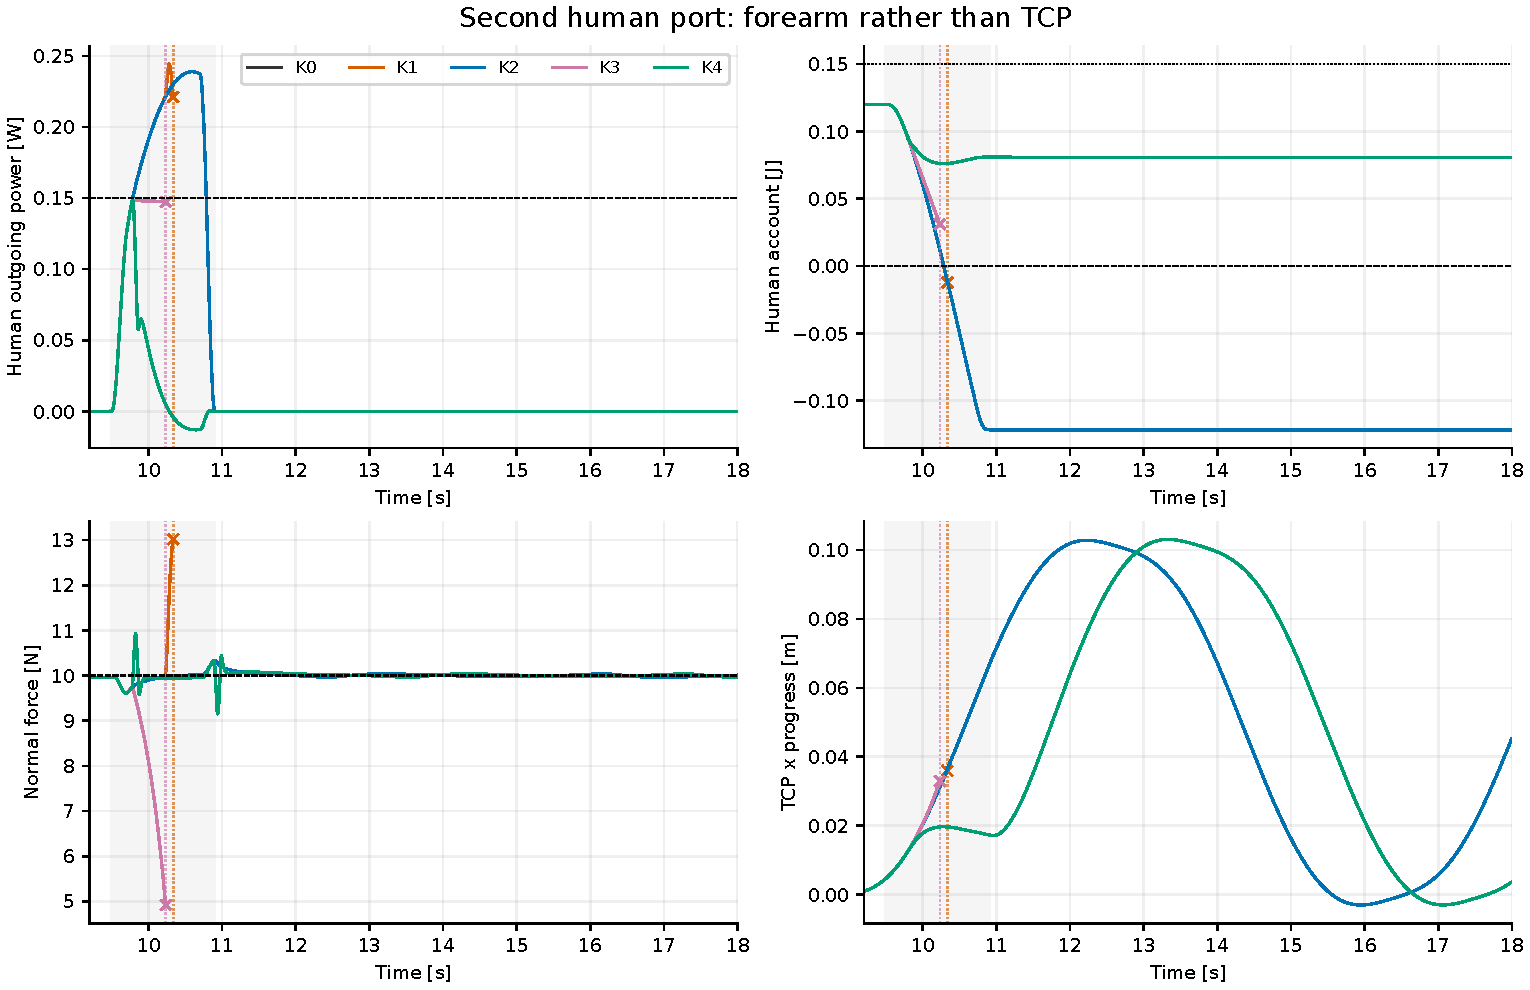
\includegraphics[width=\textwidth]{figures/fig10_forearm.pdf}
Same world-fixed blocking pulse at link5 local (0,.04,.12) m. Human power uses that actual moving point Jacobian, not TCP velocity.\par
K0: COMPLETE, end 18.000 s; net/gross H output 0.241623/0.241623 J; min H/R -0.121623/0.0583767 J; peak H 0.238858 W; measured progress 0.2453 m; QP attempts 0.\par
K1: STOP, end 10.335 s; net/gross H output 0.132274/0.132274 J; min H/R -0.0122744/0.167726 J; peak H 0.244181 W; measured progress 0.0359 m; QP attempts 242.\par
K2: COMPLETE, end 18.000 s; net/gross H output 0.241623/0.241623 J; min H/R -0.121623/0.0583767 J; peak H 0.238858 W; measured progress 0.2453 m; QP attempts 0.\par
K3: STOP, end 10.232 s; net/gross H output 0.088968/0.088968 J; min H/R 0.0310318/0.211032 J; peak H 0.148201 W; measured progress 0.0329 m; QP attempts 655.\par
K4: COMPLETE, end 18.000 s; net/gross H output 0.039143/0.043966 J; min H/R 0.076052/0.256052 J; peak H 0.148201 W; measured progress 0.2037 m; QP attempts 10.\par
\clearpage\section*{Small-budget challenge: H initialized at .001 J}
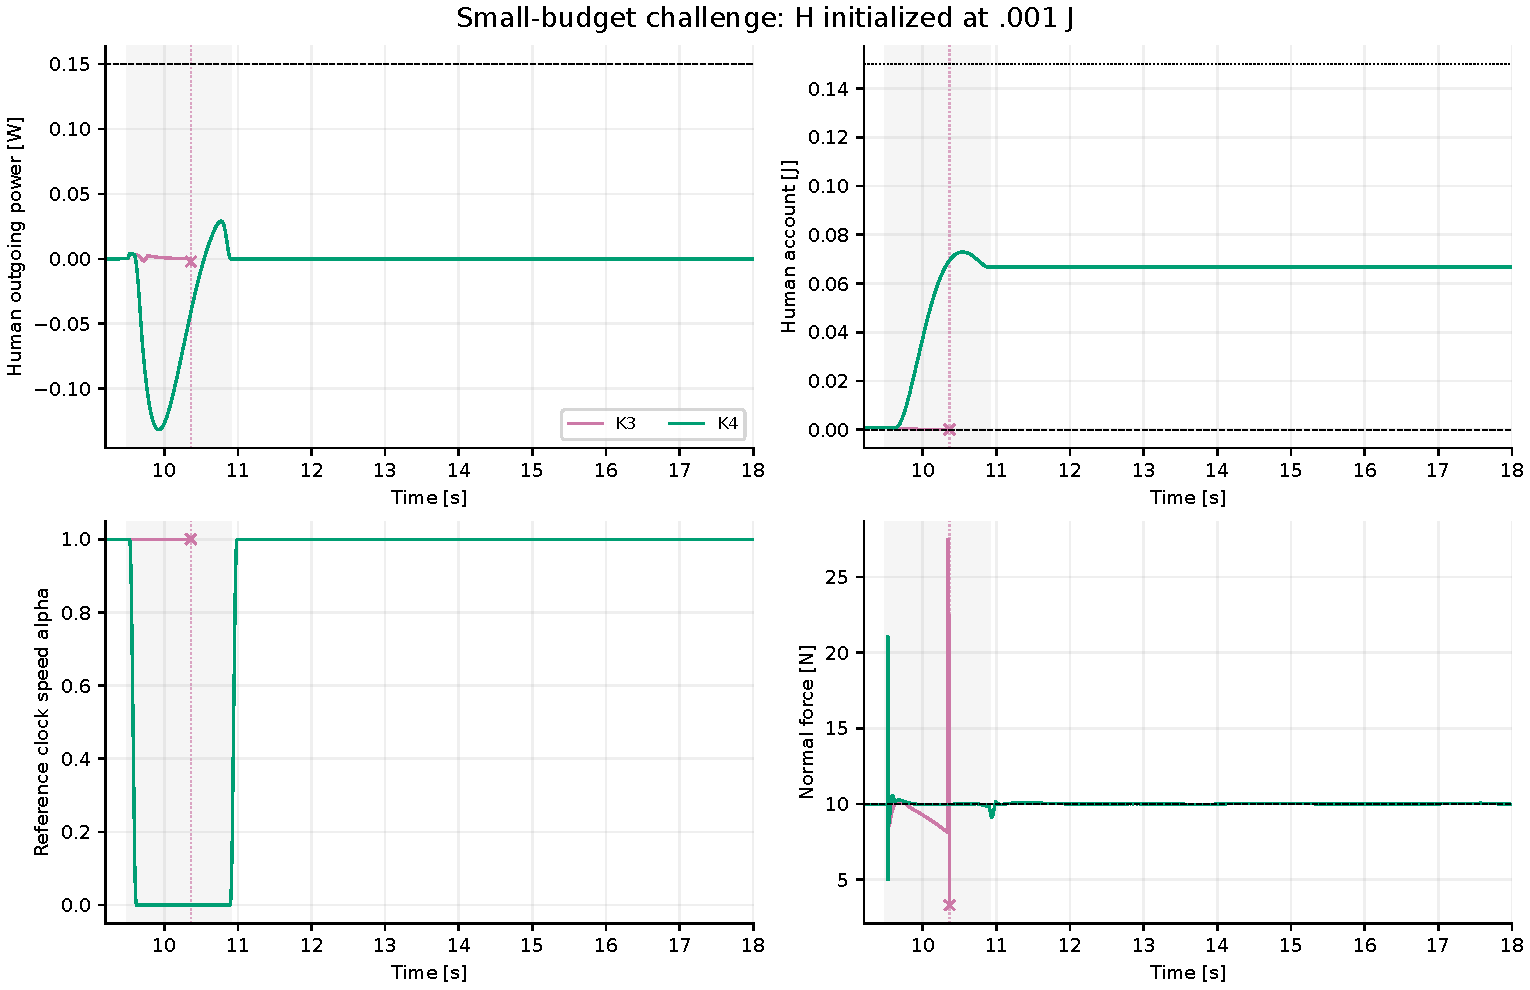
\includegraphics[width=\textwidth]{figures/fig11_starved.pdf}
Only the initial H budget changes. Explicit failures are retained with complete pre-action and failure snapshots; no safe-fallback or viability guarantee is inferred.\par
K3: STOP, end 10.363 s; net/gross H output 0.000939/0.001011 J; min H/R 5.56623e-05/0.299056 J; peak H 0.004108 W; measured progress 0.0058 m; QP attempts 1263.\par
K4: COMPLETE, end 18.000 s; net/gross H output -0.065725/0.006546 J; min H/R 0.000682986/0.293771 J; peak H 0.029066 W; measured progress 0.2009 m; QP attempts 60.\par
\clearpage\section*{Which reference claims are supported?}
\textbf{F3: avoid charging predictable task work.} K1 first filters at 10.927 s and stops at 12.541 s (nonlinear\_retries\_exhausted); K2/K3/K4 match nominal bitwise. This is accounting/filter evidence, not proof of unavoidable physical infeasibility.\par
\textbf{F4: model error appears separately.} No-human mismatch gives maximum |pR-pH|=0.084082 W and minimum R=0.067042 J; H remains .12 J. No residual intervention is required in this finite window.\par
\textbf{F5: dedicated human protection.} Residual-only K2 reaches H=-0.067435 J and 0.295100 W peak output. K4 completes with H=0.046791 J minimum and peak 0.148221 W. K3 only demonstrates a protected prefix.\par
\textbf{F6: simultaneous human and mismatch.} Executed power decomposition is independently checked for every mode. Completion and task quality must be read separately from that accounting identity.\par
\textbf{F7: bounded bidirectional charging.} K4 helping/blocking discards 0.082968 J of H charging at the .15 J cap; final H=0.068212 J. Net H output=-0.031180 J, gross=0.081788 J.\par
\textbf{F8: governor changes recovery.} K3/K4 have identical pre-governor trajectories and constraints. Primary K3 stops before release. Both K3 and K4 complete the helping/blocking case. From its 11.7 s release through 18 s, K3/K4 peak x speed is 0.056434/0.064006 m/s and maximum 10 N force error is 0.113279/1.416587 N. K4 reduces post-release reference debt from 18.303 to 13.370 mm and gross human output from 0.123659 to 0.081788 J, but increases those recovery peaks. The reference paper's smoother-recovery claim is therefore not reproduced by this governor adaptation.\par
This is deterministic simulation evidence, not a mathematical proof of general safety or reproduction of the reference paper's numerical results. Prediction uses true-plant dynamics with current measured force held for 1 ms; the task model alone is mismatched. The terminal human guard assumes force increments no greater than 60 N/s times 1 ms. Finite-difference rows are checked by fresh nonlinear rollouts; stopped cases expose solver, nonlinear acceptance, or local feasibility limits. No verified fallback, hardware execution, continuous-time certificate, or universal task-preservation claim is made. Gross outgoing energy is not bounded by a net-work account. K3/K4 have no Stage 2 reserve/backup or hard contact-quality constraints.
\end{document}
